\subsection{How it works}

As said before, our algorithm first uses Bron-Kerbosc to obtain all the maximal 
cliques of the input graph. Then, it looks for which cliques have the highest weight.
So we will explain how it does to get the different maximal cliques. \newline

The Bron-Kerbosch pivot algorithm that we used is a more efficient variant of 
the Bron-Kerbosch algorithm that is used to find all the cliques in a graph. 
It works in a similar way to the original Bron-Kerbosch algorithm, but uses a 
pivot vertex to guide the search for cliques. \newline

At each step of the algorithm, the pivot algorithm keeps track of three groups 
of vertices: the candidates, which are the set $P$ of vertices that could 
potentially be part of the clique, the already-selected vertices, which are the 
set $R$ of vertices that are definitely part of the clique, and the set $X$ of 
vertices that have been considered but not selected. \newline

The algorithm selects a pivot vertex from the set of candidates and already-selected 
vertices, and then adds to the candidate set any vertices that are connected to 
all of the vertices in the already-selected set, as well as the pivot vertex. 
It then removes from the candidate set any vertices that are not connected to all 
of the vertices in the already-selected set, and adds those vertices to the set X 
of vertices that have been considered but not selected. \newline

This process is repeated until the candidate set is empty. At that point, all of 
the vertices in the already-selected set form a clique. The algorithm is then run 
again on the remaining candidates and already-selected vertices to find any 
additional cliques. \newline

We will now illustrate it step by step with a practical example : \newline

\hspace*{1cm} \textbf{Step 0 :}
\\
\begin{minipage}{0.4\textwidth}
    \begin{tikzcd}
        6 \arrow[r, dash] & 4 \arrow[r, dash] \arrow[dd, dash] & 5 \arrow[dr, dash] \arrow[dd, dash] \\
        & & & 1 \\
        & 3 \arrow[r, dash] & 2 \arrow[ur, dash]
    \end{tikzcd}
\end{minipage}
\begin{minipage}{0.6\textwidth}
    We have here our graph as an example. As said before, the Bron-Kerbosh pivot algorithm will take 3 parameters. $R$, the set of vertices already selected. $P$, the set of candidate vertices. $X$, the set of vertices that have been considered but not selected.
\end{minipage}
Here, we have :
$$ \boxed{
        \begin{array}{lll}
            R = \{\} & P = \{1,2,3,4,5,6\} & X = \{\} \\
        \end{array}
    }$$
\\
\hspace*{1cm}  \textbf{Step 1 :}
\\
\begin{minipage}{0.4\textwidth}
    \begin{tikzcd}
        6 \arrow[r, dash] & 4 \arrow[r, dash] \arrow[dd, dash] & 5 \arrow[dr, dash] \arrow[dd, dash] \\
        & & & 1 \\
        & 3 \arrow[r, dash] & \color{red} 2 \arrow[ur, dash]
    \end{tikzcd}
\end{minipage}
\begin{minipage}{0.6\textwidth}
    Now, to begin the algorithm, we will need to chose a pivot $u$. The pivot $u$ should be chosen as one of the degree-three vertices, to minimize the number of recursive calls. Now, we suppose that $u$ is chosen to be vertex 2. We see, that there is 2 vertices that are not adjacent to 2 which are 4 and 5.
\end{minipage}
Then we know that we will work by starting with these 3 configurations (we know the first, but we don't know yet for the vertex $4$ and $6$ because some vertex could be added to $X$ or removed from $P$ when we process on $2$ or $4$) :
$$ \boxed{
        \begin{array}{lll}
            R = \{2\} & P = \{1,3,5\} & X =\{\} \\
            R = \{4\}                           \\
            R = \{6\}                           \\
        \end{array}
    }$$
\\
\hspace*{1cm}  \textbf{Step 2 :}
\\
\begin{minipage}{0.4\textwidth}
    \begin{tikzcd}
        6 \arrow[r, dash] & 4 \arrow[r, dash] \arrow[dd, dash] & \color{green} \textcircled{5} \arrow[dr, dash] \arrow[dd, dash] \\
        & & & \color{green} \textcircled{1} \\
        & \color{green} 3 \arrow[r, dash] & \color{red} \textcircled{2} \arrow[ur, dash]
    \end{tikzcd}
\end{minipage}
\begin{minipage}{0.6\textwidth}
    The algorithm begins by looking at vertex 2 in the graph. It makes a recursive call with using vertex 2 as a starting point. In this recursive call, the algorithm looks at the first group of vertices it was given (vertices 1 and 5) and selects one of them as the pivot vertex. Let's say it selects vertex 1. It then makes a first second-level recursive call for vertex 5. That will eventually find the clique $(1,2,5)$.
\end{minipage}
The recursive call process like this  :
$$ \boxed{
        \begin{array}{lll}
            R = \{2\}     & P = \{1,3,5\} & X = \{\} \\
            R = \{2,5\}   & P = \{1\}     & X = \{\} \\
            R = \{2,5,1\} & P = \{\}      & X = \{\} \\
        \end{array}
        \rightarrow P = \O \text{ and } X = \O \text{ then } (2,5,1) \text{ is a clique.}
    }$$
\\
\\
\begin{minipage}{0.4\textwidth}
    \begin{tikzcd}
        6 \arrow[r, dash] & 4 \arrow[r, dash] \arrow[dd, dash] & \color{green} 5 \arrow[dr, dash] \arrow[dd, dash] \\
        & & & \color{green} 1 \\
        & \color{green} \textcircled{3} \arrow[r, dash] & \color{red} \textcircled{2} \arrow[ur, dash]
    \end{tikzcd}
\end{minipage}
\begin{minipage}{0.6\textwidth}
    The algorithm then makes a second second-level recursive calls for vertex 3. That will eventually find the clique $(2,3)$. After these two second level recursive calls have completed, vertex 2 is added to X and removed from P.
\end{minipage}
The recursive call process like this  :
$$ \boxed{
        \begin{array}{lll}
            R = \{2\}   & P = \{1,3,5\}     & X = \{\}  \\
            R = \{2,3\} & P = \{\}          & X = \{\}  \\
            R = \{\}    & P = \{1,3,4,5,6\} & X = \{2\} \\
        \end{array}
        \rightarrow P = \O \text{ and } X = \O \text{ then } (2,3) \text{ is a clique.}
    }$$
\\
\hspace*{1cm}  \textbf{Step 3 :}
\\
\begin{minipage}{0.4\textwidth}
    \begin{tikzcd}
        \color{green} 6 \arrow[r, dash] & \color{red} \textcircled{4} \arrow[r, dash] \arrow[dd, dash] & \color{green} 5 \arrow[dr, dash] \arrow[dd, dash] \\
        & & & 1 \\
        & \color{green} \textcircled{3} \arrow[r, dash] & 2 \arrow[ur, dash]
    \end{tikzcd}
\end{minipage}
\begin{minipage}{0.6\textwidth}
    it will now do an iteration taking 4 as vertices. We note that the vertex 2 belongs to the set X in the outer call to the algorithm, but it is not a neighbor of the vertex 4 and is excluded from the subset of X passed to the recursive call. The algorithm makes a first second-level recursive call for vertex 3. That will eventually find the clique (3, 4).
\end{minipage}
The recursive call process like this  :
$$ \boxed{
        \begin{array}{lll}
            R = \{4\}   & P = \{3,5,6\} & X = \{\} \\
            R = \{4,3\} & P = \{\}      & X = \{\} \\
        \end{array}
        \rightarrow P = \O \text{ and } X = \O \text{ then } (4,3) \text{ is a clique.}
    }$$
\\
\begin{minipage}{0.4\textwidth}
    \begin{tikzcd}
        \color{green} 6 \arrow[r, dash] & \color{red} \textcircled{4} \arrow[r, dash] \arrow[dd, dash] & \color{green} \textcircled{5} \arrow[dr, dash] \arrow[dd, dash] \\
        & & & 1 \\
        & \color{green} 3 \arrow[r, dash] & 2 \arrow[ur, dash]
    \end{tikzcd}
\end{minipage}
\begin{minipage}{0.6\textwidth}
    The algorithm makes a second second-level recursive call for vertex $5$. That will eventually find the clique $(4,5)$.
\end{minipage}
The recursive call process like this  :
$$ \boxed{
        \begin{array}{lll}
            R = \{4\}   & P = \{3,5,6\} & X = \{\} \\
            R = \{4,5\} & P = \{\}      & X = \{\} \\
        \end{array}
        \rightarrow P = \O \text{ and } X = \O \text{ then } (4,5) \text{ is a clique.}
    }$$
\\
\begin{minipage}{0.4\textwidth}
    \begin{tikzcd}
        \color{green} \textcircled{6} \arrow[r, dash] & \color{red} \textcircled{4} \arrow[r, dash] \arrow[dd, dash] & \color{green} 5 \arrow[dr, dash] \arrow[dd, dash] \\
        & & & 1 \\
        & \color{green} 3 \arrow[r, dash] & 2 \arrow[ur, dash]
    \end{tikzcd}
\end{minipage}
\begin{minipage}{0.6\textwidth}
    The algorithm makes a third second-level recursive call for vertex $6$. That will eventually find the clique $(4, 6)$. After these three second level recursive calls have completed, vertex 4 is added to X and removed from P.
\end{minipage}
The recursive call process like this  :
$$ \boxed{
        \begin{array}{lll}
            R = \{4\}   & P = \{3,5,6\}   & X = \{\}    \\
            R = \{4,6\} & P = \{\}        & X = \{\}    \\
            R = \{\}    & P = \{1,3,5,6\} & X = \{2,4\} \\
        \end{array}
        \rightarrow P = \O \text{ and } X = \O \text{ then } (4,6) \text{ is a clique.}
    }$$
\\
\hspace*{1cm}  \textbf{Step 4 :}
\\
\begin{minipage}{0.4\textwidth}
    \begin{tikzcd}
        \color{red} \textcircled{6} \arrow[r, dash] & \textcircled{x} \arrow[r, dash] \arrow[dd, dash] & 5 \arrow[dr, dash] \arrow[dd, dash] \\
        & & & 1 \\
        & 3 \arrow[r, dash] & 2 \arrow[ur, dash]
    \end{tikzcd}
\end{minipage}
\begin{minipage}{0.6\textwidth}
    It will now do a third and final iteration taking 6 as vertex. It makes a recursive call but because $P$ is empty and $X$ is nom empty (the vertex $4$ was added to X and removed from P in step 3). Because of that, the algorithm immediately stops searching for cliques and backtracks, because there can be no maximal clique that includes the  vertex 6 and excludes the vertex 4.
\end{minipage}
The recursive call process like this  :
$$ \boxed{
        \begin{array}{lll}
            R = \{6\} & P = \{\} & X = \{4\} \\
        \end{array}
        \rightarrow \text{ No clique was found}
    }$$
\\
The algorithm is therefore \textbf{finished}, and we have obtained the cliques :
$$\{(2,3),(1,2,5),(3,4),(4,5),(5,6)\}$$

To summarize things and try to make things even clearer, we will take another example and make the call tree of it (the precedent example is too big) :

\begin{center}
    \begin{tikzcd}
        1 \arrow[rr, dash] \arrow[dr, dash] & & 3 \arrow[rr, dash] \arrow[dl, dash] & & 4 \\
        & 2 & & 5
    \end{tikzcd}
\end{center}
His call tree :
\begin{center}
    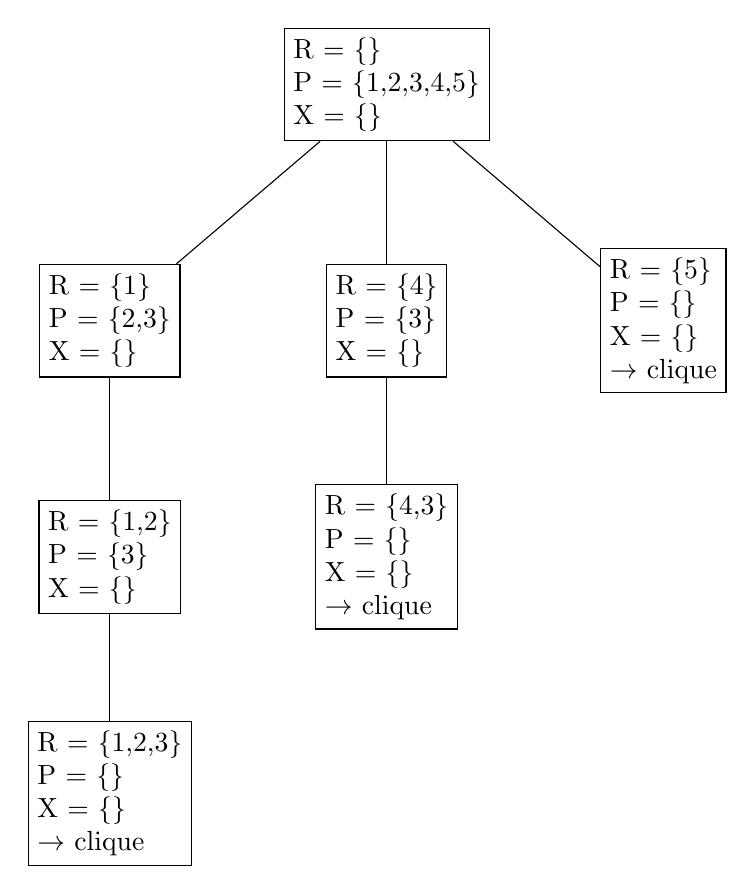
\begin{tikzpicture}[sibling distance=10em, level distance=30mm, every node/.style = {shape=rectangle, draw, align=left, top color=white}]
        \node {
            R = \{\} \\
            P = \{1,2,3,4,5\} \\
            X = \{\}
        }
        child { node {
                        R = \{1\} \\
                        P = \{2,3\} \\
                        X = \{\}
                    }
                child { node {
                                R = \{1,2\} \\
                                P = \{3\} \\
                                X = \{\}
                            }
                        child { node {
                                        R = \{1,2,3\} \\
                                        P = \{\} \\
                                        X = \{\} \\
                                        $\rightarrow$ clique
                                    }
                            }}}
        child { node {
                        R = \{4\} \\
                        P = \{3\} \\
                        X = \{\}
                    }
                child { node {
                                R = \{4,3\} \\
                                P = \{\} \\
                                X = \{\} \\
                                $\rightarrow$ clique
                            }}}
        child { node {
                        R = \{5\} \\
                        P = \{\} \\
                        X = \{\} \\
                        $\rightarrow$ clique
                    }};
    \end{tikzpicture}
\end{center}

After getting every clique, the exact algorithm will iterate all maximal clique and apply a function that will return the total weight of it.
\\ \\
This function work by iterating every possible pairs of vertices in the clique and the weight of it if there is an edge between them in a variable that start at 0. The variable will be returned as the total weight of the clique.
\\ \\
Some quick example of it :
\\ \\
\hspace*{1cm}  \textbf{Step 1 :}

\begin{center}
    Total Weight $= 0$ (start)
\end{center}

\begin{minipage}{0.4\textwidth}
    \begin{tikzcd}
        & \color{red} 1 \arrow[dl, dash, red, "3"] \arrow[dr, dash, "4"] \\
        \color{red} 2 \arrow[rr, dash, "1"] & & 3
    \end{tikzcd}
\end{minipage}
\begin{minipage}{0.6\textwidth}
    The function will take the vertex $1$ and $2$, the edge between them have a weight of $3$. It will add 3 in the variable "Total Weight".
\end{minipage}
\begin{center}
    Total Weight $= 0 + 3 = 3$
\end{center}

\hspace*{1cm}  \textbf{Step 2 :}
\\
\begin{minipage}{0.4\textwidth}
    \begin{tikzcd}
        & 1 \arrow[dl, dash, "3"] \arrow[dr, dash, "4"] \\
        \color{red} 2 \arrow[rr, dash, "1", red] & & \color{red} 3
    \end{tikzcd}
\end{minipage}
\begin{minipage}{0.6\textwidth}
    The function will take the vertex $2$ and $3$, the edge between them have a weight of $1$. It will add 1 in the variable "Total Weight".
\end{minipage}
\begin{center}
    Total Weight $= 3 + 1 = 4$
\end{center}

\hspace*{1cm}  \textbf{Step 3 :}
\\
\begin{minipage}{0.4\textwidth}
    \begin{tikzcd}
        & \color{red} 1 \arrow[dl, dash, "3"] \arrow[dr, dash, red, "4"] \\
        2 \arrow[rr, dash, "1"] & & \color{red} 3
    \end{tikzcd}
\end{minipage}
\begin{minipage}{0.6\textwidth}
    The function will take the vertex $1$ and $3$, the edge between them have a weight of $4$. It will add 4 in the variable "Total Weight".
\end{minipage}
\begin{center}
    Total Weight $= 4 + 4 = 8$
\end{center}

The total weight of this clique is 8.
\\ \\
The algorithm then takes the clique with the greatest weight. And \textbf{the MEWC is solved}.
